\section{Svolgimento}

È stato definita l'architettura generale del sistema.

Vengono definite le seguenti componenti:



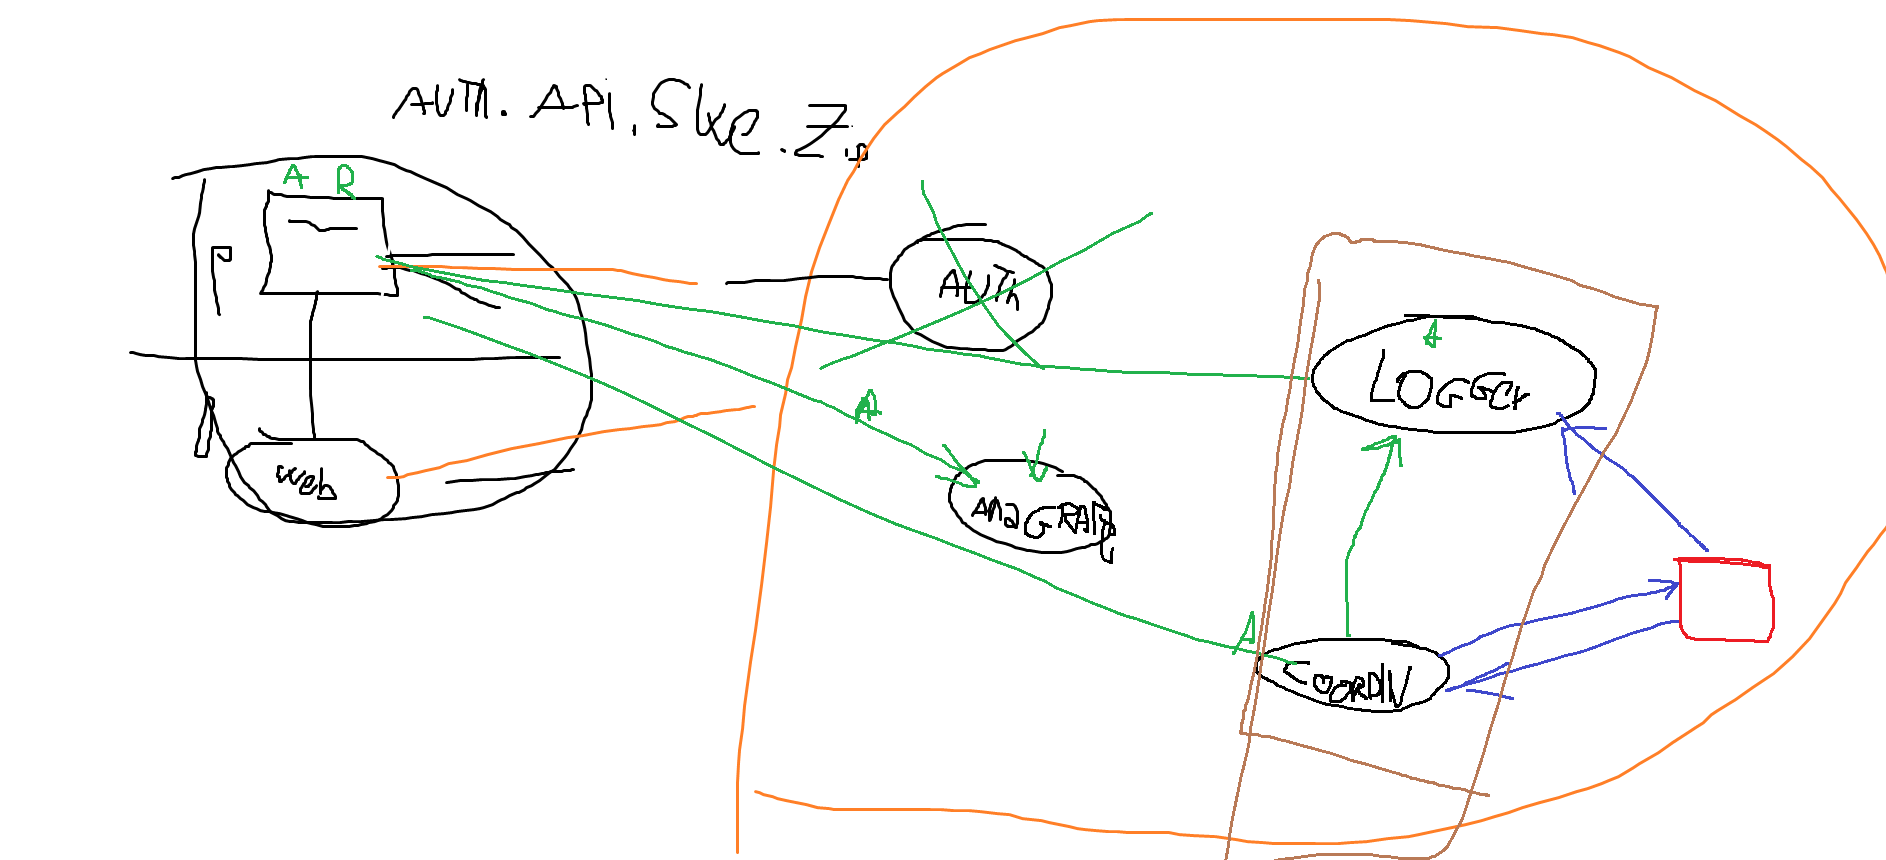
\includegraphics[width = 0.9\linewidth]{img/architettura.png}

\begin{itemize}
    \item \textbf{Client}: interfaccia grafica per l'utente;
    \item \textbf{Authentication microservice}: gestisce l'autenticazione degli utenti;
    \item \textbf{Anagraphic microservice}: gestisce la parte anagrafica dei lamponi;
    \item \textbf{Data microservice}: gestisce la parte di raccolta e analisi dati;
    \item \textbf{Coordinator microservice}: gestisce l'accensione e lo spegnimento delle aree illuminate a seconda di logiche interne;
\end{itemize}

Sono presenti inoltre in supporto:
\begin{itemize}
    \item \textbf{Database}: database per la memorizzazione dei dati;
    \item \textbf{Message broker}: gestisce la comunicazione tra i lampioni, il sistema di raccolta dati e il sistema di coordinamento;
\end{itemize}

Tutto questo definisce una REST-based topology.